% To add an image or include a .tex file you need to add
% \CWD
% to the relative (to the main document) path.
%
% Example:
% \begin{figure}
%   \centering
%   \includegraphics{\CWD/images/example.pdf}
% \end{figure}

Emanuel estava estudando Programação Competitiva, resolvendo problemas sobre palíndromos. Um palíndromo é uma string que permanece igual quando lida de trás para frente, como {\tt arara} e {\tt tenet}. Além disso, Emanuel sabe que uma substring de uma string $T$ é uma string que pode ser obtida apagando-se caracteres do início e fim de $T$. Por exemplo, {\tt ara}, {\tt ar} e {\tt arara} são substrings de {\tt arara}.

Ao se deparar com o problema clássico de computar quantas substrings de uma string $S$ são palíndromos, Emanuel se perguntou como que esse problema poderia ser resolvido se pudessemos re-ordenar cada substring. Ou seja, dado uma string $S$, quantas substrings de $S$ (contando repetições) podem ser re-ordenadas para formar um palíndromo.

\begin{figure}[H]
    \centering
    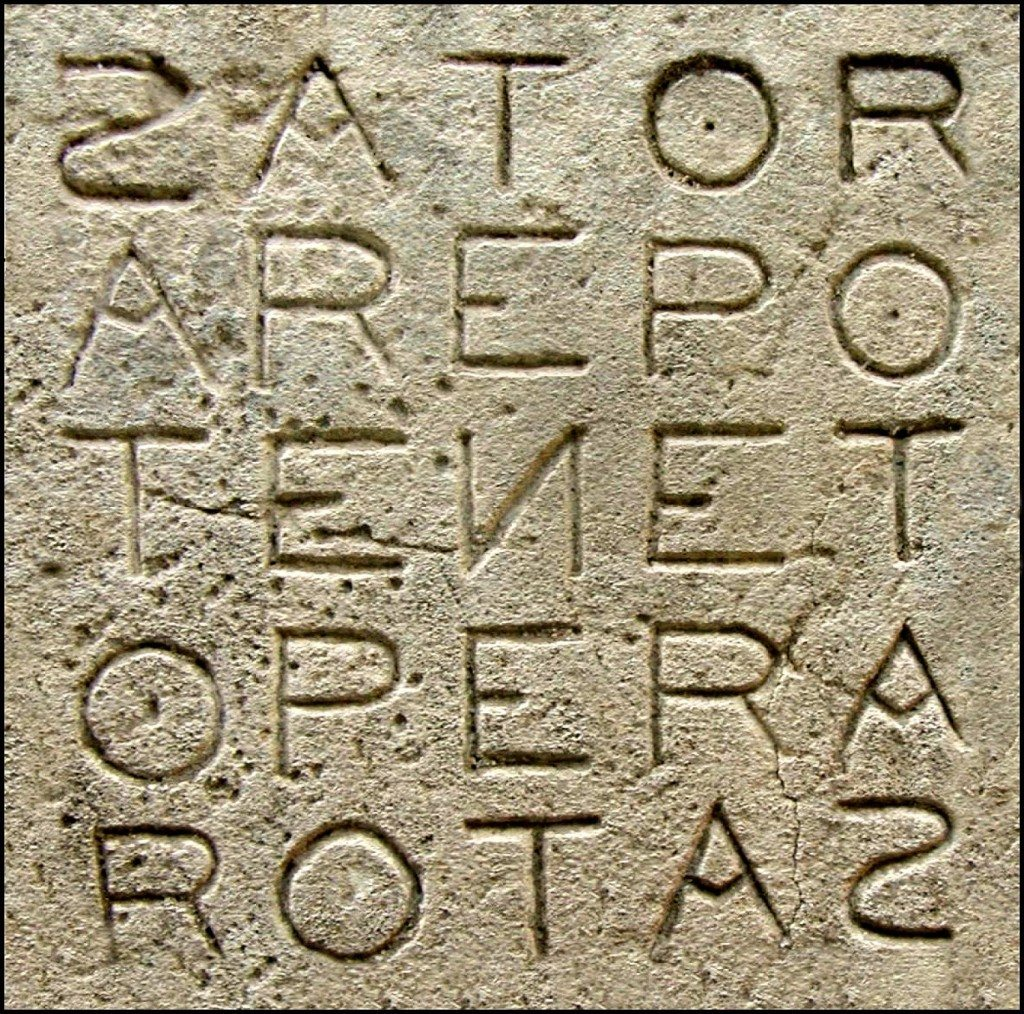
\includegraphics[width=5cm]{\CWD/tenet.jpg}
\end{figure}

Cansado após implementar o problema clássico, Emanuel pede sua ajuda para implementar a variação descrita acima para ele. Para simplificar o problema para você, ele garante que a string nunca conterá vogais ({\tt a}, {\tt e}, {\tt i}, {\tt o}, {\tt u}, {\tt y}).

%
% For input, use one of the following
%
\inputdesc{A primeira linha contém um inteiro $N$ onde $1 \leq N \leq 10^6$.}
\inputdesc{A segunda linha contém uma string $S$ com $N$ caracteres. $S$ é composta por letras minúsculas e não possui os caracteres {\tt a}, {\tt e}, {\tt i}, {\tt o}, {\tt u}, {\tt y}.}

%
% For output, use one of the following
%

\outputdesc{Imprima um único inteiro: o número de substrings de $S$ que podem ser re-ordenadas para formar um palíndromo.}

%\sampleio will look for files named sample-n.in and sample-n.sol (where n is 1, 2, 3...)
%in the documents directory and include them as samples.

\section*{Restrições}

\begin{itemize}
\item $1 \leq N \leq 10^6$.
\end{itemize}

\sampleio

\bigskip
\textbf{Explicação do Exemplo 1}: As 12 substrings são:

% eennt
\begin{multicols}{2}
\begin{enumerate}
	\item {\tt f}
	\item {\tt f}
	\item {\tt g}
	\item {\tt g}
	\item {\tt h}
	\item {\tt ff}
	\item {\tt gg}
	\item {\tt ffg}
	\item {\tt fgg}
	\item {\tt ggh}
	\item {\tt ffgg}
	\item {\tt ffggh}
\end{enumerate}
\end{multicols}
